\documentclass{article}

\usepackage[T1]{fontenc}
\usepackage[polish]{babel}
\usepackage{graphicx}
\usepackage[section]{placeins}

\title{Klasyfikowanie dokumentów - program typu Manager - Workers\large \\
Systemy równoległe i rozproszone}
\author{Łukasz Wajda, Mariusz Biegański} 

\begin{document}
\maketitle

\section{Opis projektu}
W internecie jest wile dokumentów, aby znaleźć właściwy dokument za pomocą wyszukiwarki wymyślono algorytm zliczający ilość słów w dokumentach i zapisujący to w postaci wektora. Projekt wykorzystuje rozmaite pliki tekstowe łatwe do przetwarzania takie jak .txt, .odt, .css, .html, .xml. Korzystając z pliku zawierającego listę słow, tzw. słownik tworzymy wektor zawierający ilość wystąpnień danego słowa dla każdego pliku. Na koniec wyniki zapisujemy do pliku.

\section{Opis budowy programu}
Program został napisany z wykorzystaniem biblioteki MPI (Message Passing Interface). Składa się z trzech funkcji: \textit{main}, \textit{manager} i \textit{worker} oraz enum \textit{Tags} do reprezentacji stałych wartości.

\section{Opis działania programu}
\subsection{Funkcja \textit{main}}
Inicjalizujemy MPI i uzyskujemy informacje o liczbie procesów i identyfikatorze bieżącego procesu. Następnie tworzony jest komunikator worker\_communicator, który będzie używany do komunikacji między menadżerem a workerami. Jeśli identyfikator procesu wynosi 0 (czyli jest to menadżer), przypisuje się proces do komunikatora o kolorze undefined za pomocą funkcji \textit{MPI\_Comm\_split}, po to aby nie komunikował się tak jak worker. Następnie wywołuje funkcję manager przekazując jej argumenty argc, argv oraz liczbę procesów num\_processes. W przeciwnym razie, jeśli identyfikator procesu nie jest równy 0 (czyli jest to worker), funkcja main wywołuje \textit{MPI\_Comm\_split} dla komunikatora \textit{MPI\_COMM\_WORLD}, tworząc nowy komunikator worker\_communicator dla workerów o kolorze 0. Następnie wywołuje funkcję worker przekazując jej argumenty argc, argv oraz komunikator worker\_communicator. Na końcu funkcja main wywołuje \textit{MPI\_Finalize} w celu zamknięcia środowiska MPI i zwraca wartość 0.

\subsection{Funkcja \textit{manager}}
Na początku zostaje wywołana asynchroniczna funkca czekająca na dowolny proces, który prześle informację o ilości słów w słowniku otagowaną \textit{DICTIONARY\_SIZE\_MESSAGE}. Podczas czekania manager przeszukuje podany folder i zapisuje nazwy plików do wektora napisów. Po wczytaniu listy program jest blokowany i czeka na zakończenie funkcji asynchronicznej. Następnie alokowane jest potrzebne miejsce na wyniki zwrócone przez funkcje \textit{worker} z liczbą wystąpień słow w danym pliku. Po zaalokowaniu pamięci wykonuje się pętla while do czasu zakończenia pracy wszystkich funkcji \textit{worker}. W pętli manger czeka na wiadomość od workera. Jeśli jest ona otagowana \textit{FILE\_VECTOR\_MESSAGE} to wynik zostaje dodany do zmiennej przechowującej wektory wystąpień dla każdego pliku. Dalej w pętli sprawdza się czy liczba przypisanych plików jest mniejsza od całkowitej liczby plików, jeśli tak to przesyłana zostaje nazwa pliku do funkcji \textit{worker}, w przeciwnym przypadku zostaje przesłany komunikat do \textit{worker} o końcu pracy. Po zakończeniu pętli wyniki zostają zapisane do pliku \textit{result.txt}.

\subsection{Funkcja \textit{worker}}
Funkcja pobiera swój identyfikator procesu, następnie wysyła pusty komunikat informujący o gotowości do pracy. Jeśli worker ma identyfikator równy zero to wczytuje słownik z pliku i koduje go tablicy charów oddzielając słowa znakiem '|'. Następnie rozmiar słownika zostaje rozgłoszony funkcją \textit{MPI\_Bcast}. Pozostałe workery używają otrzymanej długości słownika do zaalokowania pamięci na słownik. Następnie zostaje rozgłoszony zakodowany słownik do pozostałych workerów. Workery o indeksie różnym od zera dekodują otrzymany słownik i zapisują do wcześniej zaalokowanej zmiennej. Po rozgłoszeniu słownika worker o indeksie zero przesyła do managera ilość słów w słowniku. Na koniec wykonuję się nieskończona pętla while, w której worker sprawdza czy jest dostępna wiadomość otagowana \textit{SOURCE\_FILE\_MESSAGE} za pomocą funkcji \textit{MPI\_Probe}. Jeśli tak to pobierana jest długość nazwy pliku do przetworzenia. W przypadku gdy długość nazwy wynosi zero pętla zostaje przerwana i kończy się funkcja. Po uzyskaniu długości nazwy zostaje pobrana nazwa pliku, a następnie zapisana do lokalnej zmiennej. Plik zostaje wczytany, stworzony zostaje wektor wystąpień, który jest przesyłany do funkcji \textit{manager}. Po zakończeniu pętli zostają zwolnie zasoby.

\begin{figure}[!htb]
  \centering
  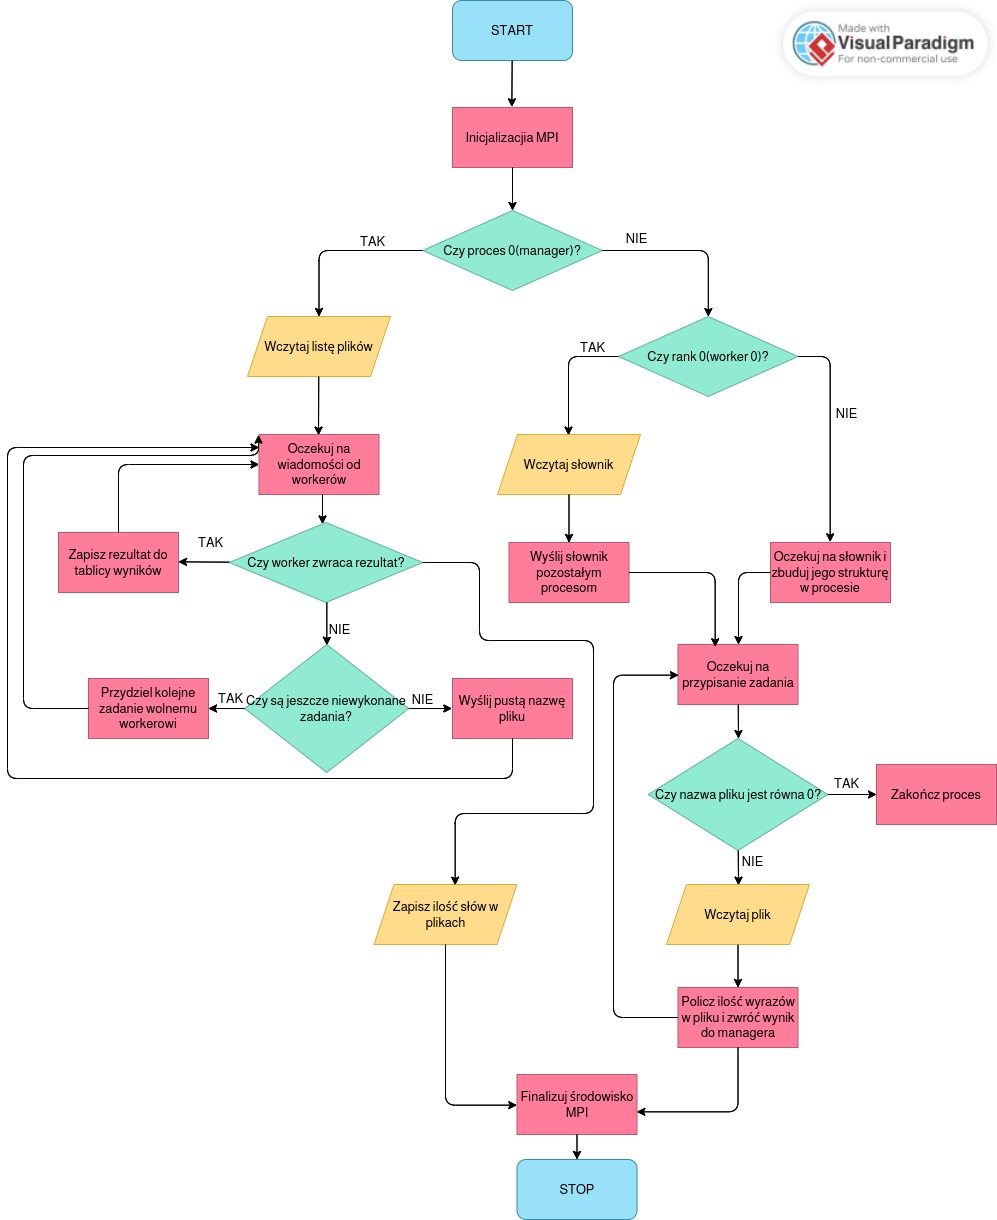
\includegraphics[width=\textwidth]{diagram.jpg}
  \caption{Schemat blokowy}
  \label{fig:diagram}
\end{figure}
\

\section{Obsługa programu}
Program kompilujemy poleceniem \textit{make}, uruchamiamy poleceniem \textit{make run}, a czyścimy projekt do stanu początkowego poleceniem \textit{make clean}.\\
Słownik znajduje się w pliku \textit{data/checkedWords.txt} i można go modyfikować. Dodatkowo można dodawać i usuwać pliki tekstowe do sprawdzenia w folderze data.
Wynik można wyświetlić w terminalu za pomocą komendy \textit{cat result.txt}, należy pamiętać by wyświetlić wynik po uruchomieniu programu i przed przywróceniem projektu do stanu początkowego.
Przykładowy wynik znajduje się w pliku example.txt i można go wyświetlić w terminalu za pomocą komendy \textit{cat example.txt}.

\end{document}
